\chapter{Návrh a specifikace funkcionalit}\label{chap:navrh-a-specifikace}

Hlavním důvodem pro implementaci přidaných funkcionalit formou rozšíření do webových prohlížečů byla nemožnost přímo zasahovat do školního informačního systému InSIS. Toto omezení je způsobeno tím, že informační systém InSIS je pro VŠE v~Praze dodávaný externí firmou IS4U, s.r.o. se sídlem v~Brně, jako řešení nejen bez zdrojových kódů, ale také bez veřejného API. 

Rozšíření do webových prohlížečů jsou softwarové balíčky, které mění nebo rozšiřují funkce webových prohlížečů a umožňují strojovou interakci s~webovými stránkami, které uživatel webového prohlížeče navštěvuje \cite{web_extensions_2019}\footnote{Autorem všech překladů z~angličtiny je autor práce}. Všechny populární webové prohlížeče mají zabudovanou podporu pro webová rozšíření a v~posledních letech byla vyvinuta snaha o~unifikaci aplikačního rozhraní pro vývoj a spouštění těchto rozšíření, aby byla zajištěna lepší kompatibilita napříč různými webovými prohlížeči.  

Alternativou pro webové rozšíření by byly již v~úvodu zmíněné uživatelské skripty, které ale vyžadují instalaci hostitelského prostředí a následnou instalaci ze zdrojových souborů. To je pro značnou část uživatelů méně přívětivou variantou, protože instalace uživatelského skriptu je podstatně pracnější a technicky náročnější než instalace rozšíření do webového prohlížeče. 

Před implementací rozšíření do webových prohlížečů a podpůrného webového serveru je potřeba vymezit o~jaké funkcionality by se měl školní informační systém InSIS rozšířit. 
Hlavním zdrojem pro výběr funkcionalit k~implementaci byly potřeby autora a konzultace se spolužáky, ze kterých byly vypozorovány opakující se problémy a často zmiňovaná slabá místa informačního systému InSIS. 

Jedním z~nejčastěji zmiňovaných nedostatků je modul odevzdávárny, pomocí kterého studenti během svého studia nahrávají a~odevzdávají soubory, například domácí úkoly nebo seminární práce. Je časté, že vyučující vypíše všechny odevzdávárny již na začátku semestru a~je pak odpovědností studentů hlídat, kterým odevzdávárnám se blíží datum uzavření. Z~konzultací s~ostatními uživateli informačního systému InSIS vyplynulo, že studenti tento problém řeší 2 způsoby: první skupina lidí používá synchronizaci dostupných událostí s~Outlook kalendářem nebo Google kalendářem a~ocenili by možnost exportovat si datum uzavření odevzdávárny do kalendáře. Druhá, podstatně početnější skupina lidí, která synchronizaci s~kalendářem nepoužívá, by naopak ocenila možnost nechat si zaslat na email upozornění na odevzdávárny s~blížícím se datem uzavření. Tuto funkcionalitu dále popisuje kapitola \ref{sec:pripomenuti-odevzdavaren}.

\section{Přihlášení pomocí školního účtu}

Aby bylo možné bezpečně uchovávat uživatelská data na podpůrném serveru, je nutné navrhnout a implementovat přihlášení do rozšíření. Přihlášení je možné pomocí emailové adresy na doméně \url{vse.cz}, protože každý uživatel, který pracuje se školním informačním systémem \mbox{InSIS}, již takovou emailovou adresu vlastní a~tato adresa je zároveň unikátním identifikátorem každého uživatele. Bylo proto navrženo autentikační schéma, které využívá pro přihlášení školní emailovou adresu bez nutnosti předchozí registrace.
Celý proces přihlášení uživatele je zachycen pomocí diagramu na obrázku \ref{fig:autentikace}.

Grafické rozhraní pro přihlašování bylo navrženo jako formulář, který obsahuje 2 části, kde v~první části je zobrazené uživatelské rozhraní pro zadání školní emailové adresy a po zadání školní emailové adresy se zobrazí druhá část, kde je zobrazené uživatelské rozhraní pro zadání kódu zaslaného na emailovou adresu zadanou v~předchozí části.
Návrh grafického rozhraní formuláře pro přihlášení zachycuje obrázek \ref{fig:autentikace-wireframe} a obrázek \ref{fig:usecase-prihlaseni} zachycuje diagram případů užití pro funkcionalitu přihlášení do rozšíření.

\begin{figure}[htbp!]\centering
    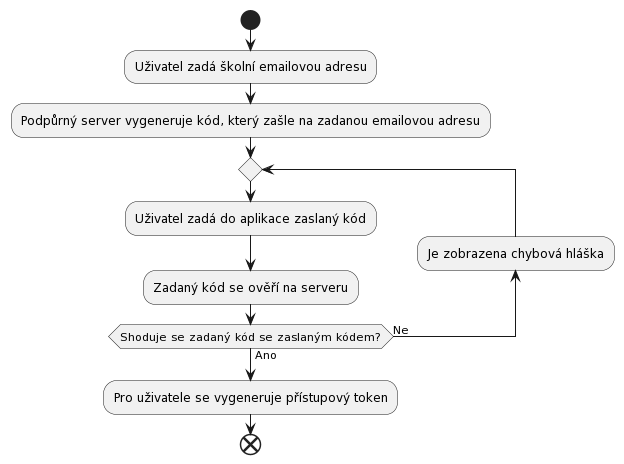
\includegraphics[width=\textwidth]{img/autentikace.png}
    \caption{Vývojový diagram přihlášení uživatele (vlastní zpracování)}
    \label{fig:autentikace}
\end{figure}
\imgsource{
@startuml
start
:Uživatel zadá školní emailovou adresu;
:Podpůrný server vygeneruje kód, který zašle na zadanou emailovou adresu;
repeat 
    :Uživatel zadá do aplikace zaslaný kód;
    :Zadaný kód se ověří na serveru;
backward :Je zobrazena chybová hláška;
repeat while (Shoduje se zadaný kód se zaslaným kódem?) is (Ne) not (Ano)
:Pro uživatele se vygeneruje přístupový token;
end
@enduml
}


\begin{figure}[htbp!]\centering
    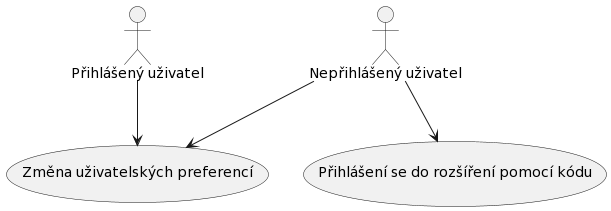
\includegraphics[width=\textwidth]{img/uc-prihlaseni.png}
    \caption{Diagram případů užití přihlášení (vlastní zpracování)}
    \label{fig:usecase-prihlaseni}
\end{figure}
\imgsource{
@startuml
"Přihlášený uživatel" as user
"Nepřihlášený uživatel" as anonymous

user --> (Změna uživatelských preferencí)
anonymous --> (Změna uživatelských preferencí)
anonymous --> (Přihlášení se do rozšíření pomocí kódu)
@enduml
}

\begin{figure}[htbp!]\centering
    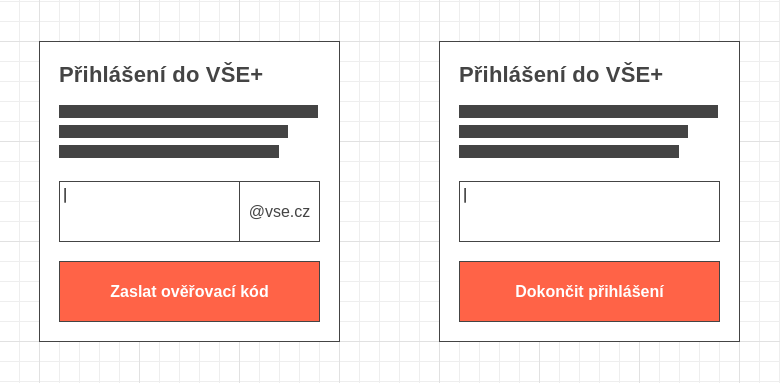
\includegraphics[width=\textwidth]{img/wireframe-autentikace.png}
    \caption{Návrh grafického rozhraní přihlášení uživatele (vlastní zpracování)}
    \label{fig:autentikace-wireframe}
\end{figure}


\section{Zobrazení náhledu rozvrhu při registracích předmětů}

První funkcionalitou, kterou webové rozšíření do informačního systému InSIS přidává, je zobrazení náhledu rozvrhu a detekce kolizí se zapsanými hodinami při registraci rozvrhových akcí. V~uživatelském rozhraní pro registraci rozvrhových akcí nejsou v~informačním systému InSIS zobrazené již zaregistrované rozvrhové akce a je tedy velice obtížné si efektivně sestavovat rozvrh. Většina dotazovaných studentů tento nedostatek řeší tak, že si registrují předměty za pomoci kombinace dvou oken prohlížeče, kdy v~jednom okně mají otevřený rozvrh a v~druhém okně mají otevřené registrace předmětů. Kolize studenti hledají manuálně, často až pomocí vizuální kontroly po registraci rozvrhové akce.

Efektivitu uživatelů systému InSIS při registraci rozvrhových akcí je možné zlepšit zobrazením náhledu rozvrhu s~již zaregistrovanými rozvrhovými akcemi vedle seznamu dostupných rozvrhových akcí pro předmět, který si uživatel aktuálně zapisuje. Další zlepšení efektivity pak poskytuje automatická detekce kolizí v~rozvrhu a vizuální odlišení hodin s~kolizí ve výběru dostupných rozvrhových akcí. Toto odlišení může být implementováno například jako zvýšení průhlednosti řádků v~tabulce. 

Při zápisu rozvrhových akcí při registracích předmětů je celý obsah stránky zarovnaný na levou stranu obrazovky a při zápisu u~většiny rozvrhových akcí formulář pro výběr dne a času nezabírá ani polovinu dostupného místa na obrazovce. Proto je vhodné implementovaný náhled rozvrhu s~již zaregistrovanými rozvrhovými akcemi umístit do pravé části obrazovky.

Celý funkční proces pro náhled rozvrhu při registraci rozvrhových akcí popisuje diagram zobrazený na obrázku \ref{fig:wireframe-timetable-preview}.

\begin{figure}[htbp!]\centering
    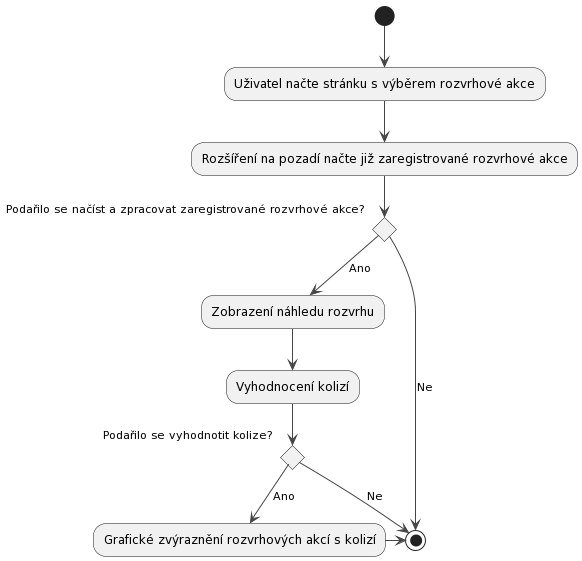
\includegraphics[width=\textwidth]{img/flow-timetable-preview.png}
    \caption{Vývojový diagram popisující funkcionalitu náhledy rozvrhů (vlastní zpracování)}
    \label{fig:wireframe-timetable-preview}
\end{figure}
\imgsource{
    @startuml
    (*) --> "Uživatel načte stránku s~výběrem rozvrhové akce"
    
    --> "Rozšíření na pozadí načte již zaregistrované rozvrhové akce"
    
    if "Podařilo se načíst a zpracovat zaregistrované rozvrhové akce?" then
      -->[Ano] "Zobrazení náhledu rozvrhu"
      --> "Vyhodnocení kolizí"
      if "Podařilo se vyhodnotit kolize?" then
        -->[Ano] "Grafické zvýraznění rozvrhových akcí s~kolizí"
        -right-> (*)
      else
         -right->[Ne] (*)
      endif
    else
      -right-->[Ne](*)
    endif
    @enduml
}

\section{Připomenutí odevzdáváren a export do externího kalendáře}\label{sec:pripomenuti-odevzdavaren}

Nedílnou součástí školního informačního systému InSIS je modul odevzdávárny. Tento modul slouží pro nahrávání a odevzdávání souborů a je nejčastěji využíván vyučujícími jako prostředek pro sběr vypracovaných domácích úkolů a seminárních prací. 

Jedním z~vypozorovaných nedostatků je absence možnosti si na odevzdávárnu nechat zaslat upozornění. Informační systém InSIS podobnou funkcionalitu u~některých jiných modulů nabízí. Příkladem může být funkce hlídací pes při přihlašování se na termíny zkoušek, pomoíc které si student může nechat zaslat oznámení na email v~případě, že se uvolní místo na vybraném termínu.

Tento nedostatek umocňuje skutečnost, že řada vyučujících vypisuje odevzdávárny pro celý semestr již během prvního týdne a je pak častým problémem, že student na některé z~pozdějších odevzdáváren zapomene, jelikož datum vypsání a datum uzavření mohou být od sebe i v~řádech několika měsíců.

Dalším potencionálním zlepšením práce uživatelů s~odevzdávárnami je možnost exportu a synchronizace datumů uzavření s~kalendářem. Podobně jako u~připomenutí, tato funkcionalita je dostupná v~několika jiných modulech informačního systému InSIS. Jedním z~příkladů může být opět modul pro přihlašování na termíny zkoušek, který umožňuje synchronizaci časů zkoušek s~kalendářem.

Obrázek \ref{fig:usecase-odevzdavarny} zachycuje diagram případů užití pro jednotlivé funkcionality připomenutí odevzdáváren.

\begin{figure}[htbp!]\centering
    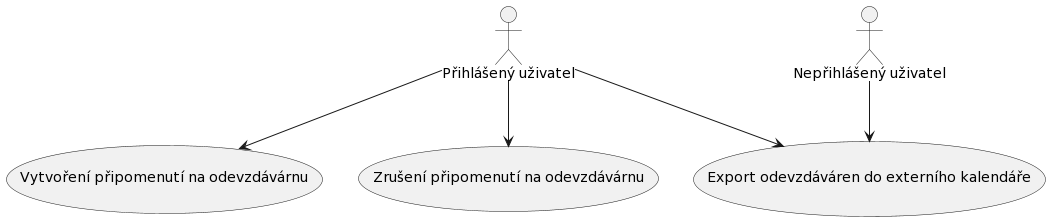
\includegraphics[width=\textwidth]{img/uc-odevzdavarny.png}
    \caption{Diagram případů užití připomenutí odevzdáváren (vlastní zpracování)}
    \label{fig:usecase-odevzdavarny}
\end{figure}
\imgsource{
@startuml
"Přihlášený uživatel" as user
"Nepřihlášený uživatel" as anonymous

user --> (Vytvoření připomenutí na odevzdávárnu)
user --> (Zrušení připomenutí na odevzdávárnu)
user --> (Export odevzdáváren do externího kalendáře)
anonymous --> (Export odevzdáváren do externího kalendáře)
@enduml
}

\subsection{Návrh rozložení prvků na stránce}

Z~analýzy grafického rozložení modulu pro odevzdávárny, že adekvátním řešením integrace uživatelského rozhraní pro připomínání odevzdáváren a export do externího kalendáře bude využití prázdného místa na pravé straně obrazovky rozšířením tabulky s~otevřenými odevzdávárnami o~2 nové sloupce.

Rozšířené nastavení připomenutí pro konkrétní odevzdávárnu bude implementováno v~podobě dialogového okna, které se otevře až po kliknutí na ikonu v~rozšířené tabulce. Tímto způsobem je možné schovat komplexní uživatelské rozhraní pro výběr časů a správu připomenutí až do chvíle, kdy je to pro uživatele systému přínosné a relevantní. 

\subsection{Export do kalendáře}

Podnět pro implementaci exportu času a předmětu odevzdáváren do externího kalendáře přišel od jednoho ze studentů, který stejně jako část dalších studentů na Vysoké škole ekonomické v~Praze, využívá synchronizaci rozvrhu se školním kalendářem Microsoft Outlook z~balíčku Microsoft Office 365.

Tato synchronizace se školním kalendářem podporuje kromě přímé synchronizace rozvrhových akcí v~rámci týdne i propisování datumů a časů zkoušek, na které je student přihlášen. Jednou z~informací, která v~tomto exportovaném kalendáři chybí jsou datumy a časy uzavření vypsaných odevzdáváren.

Po vyhodnocení dotazníkového šetření s~celkovým počtem 31 respondentů byly jako podporované externí kalendáře s~největším počtem respondentů zvoleny produkty Google Calendar a Microsoft Outlook.

\section{Vylepšený rozvrh}\label{sec:vylepseny-rozvrh}

Poslední z~navržených funkcionalit je vylepšená verze rozvrhu. Tato vylepšená verze se od původní verze liší jak po grafické, tak po funkční stránce. Nejzásadnějším rozdílem je integrace konceptu přepínání mezi jednotlivými výukovými týdny v~rámci rozvrhu. Původní implementace rozvrhu poskutovaná informačním systémem InSIS zobrazuje pouze statický rozvrh, který není závislý na aktuálně probíhajícím výukovém týdnu. 

Obrázek \ref{fig:usecase-rozvrh} zachycuje diagram případů užití pro jednotlivé funkcionality vylepšeného rozvrhu.

\begin{figure}[htbp!]\centering
    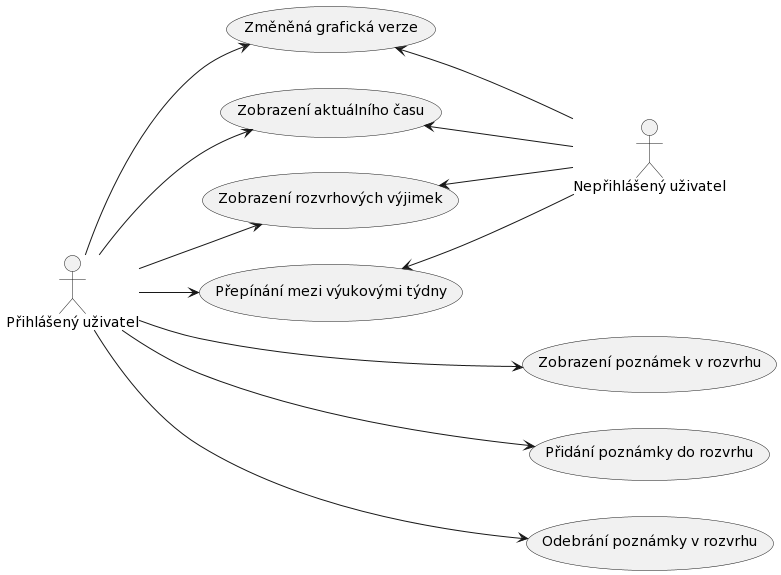
\includegraphics[width=\textwidth]{img/uc-rozvrh.png}
    \caption{Diagram případů užití vylepšeného rozvrhu (vlastní zpracování)}
    \label{fig:usecase-rozvrh}
\end{figure}
\imgsource{
@startuml
left to right direction
"Přihlášený uživatel" as user
"Nepřihlášený uživatel" as anonymous

user --> (Změněná grafická verze)
user --> (Zobrazení aktuálního času)
user --> (Zobrazení rozvrhových výjimek)
user --> (Přepínání mezi výukovými týdny)


user ---> (Zobrazení poznámek v~rozvrhu)
user ---> (Přidání poznámky do rozvrhu)
user ---> (Odebrání poznámky v~rozvrhu)

(Změněná grafická verze) <-- anonymous
(Zobrazení aktuálního času) <-- anonymous
(Zobrazení rozvrhových výjimek) <-- anonymous
(Přepínání mezi výukovými týdny) <-- anonymous
@enduml
}

\subsection{Změněný vzhled rozvrhu}

Jelikož v~rámci implementace bude docházet k~sestavování nové DOM stromové reprezentace pro zobrazení komponent tvořících zobrazení rozvrhu, naskytuje se příležitost vylepšit grafickou stránku rozvrhu. 

Pro vylepšenou verzi rozvrhu byla zvolena nová paleta barev, bylo změněno rozložení dílčích informací zobrazených v~buňkách reprezentujících rozvrhové akce a u~každé rozvrhové akce byl dále přidán explicitní čas začátku a konce. Poslední změnou je úprava mezer vně kontejneru pro zobrazení informací a úprava typografických vlastností textu pro zajištění lepší čitelnosti a zjednodušení orientace v~rozvrhu.

\subsection{Přepínání mezi týdny a zpracování rozvrhových výjimek}

Klíčovou změnou ve vylepšené verzi rozvrhu je práce s~jednotlivými výukovými týdny. To zahrnuje zobrazení aktuálního týdne v~záhlaví rozvrhu společně s~uživatelským rozhraním pro přepínání mezi týdny. Dále oproti původní implementaci rozvrhu probíhá navíc zpracování výjimek v~rozvrhových akcích, které jsou tvořeny zejména volnými dny, ve kterých výuka odpadá a dny, ve kterých probíhají blokové akce. Pokud v~konkrétním týdnu rozvrhová akce neprobíhá, je rozvrhová akce v~rozvrhu graficky odlišena. Toto grafické odlišení poskytuje uživateli zrychlenou zpětnou vazbu oproti původní číselné poznámce pod rozvrhem, kterou je možné snadno přehlédnout.

Během zpracování poznámek v~rozvrhu dochází k~detekci začátku a konce výukového období, které je následně v~uživatelském rozhraní pro přepínání týdnů využito pro zobrazení pořadového čísla týdne, a jestli je tento týden součástí výukového období.

\subsection{Zobrazení aktuálního času v~rozvrhu}

Další přidanou funkcionalitou do zobrazení rozvrhových akcí je vyznačení aktuálního času přímo v~rozvrhu. Cílem této funkcionality je podobně jako u~zpracování výjimek rozvrhových akcí zlepšit zpětnou vazbu pro uživatele informačního systému, protože vyznačení aktuálního času v~rozvrhu zlepšuje navigaci a snižuje čas pro nalezení aktuálně probíhající hodiny. 

\subsection{Možnost přidání poznámek ke konkrétním hodinám}

Poslední přidanou funkcionalitou, která rozšiřuje funkce rozvrhu je možnost přidávání poznámek ke konkrétním hodinám. To je užitečné zejména pro označení naplánovaných průběžných testů, domácích úkolů nebo prezentací. 

Z~konzultací s~ostatními studenty vyplynulo, že značná část dotazovaných studentů sdílí workflow pro přípravu na nadcházející týden s~autorem práce. Tento workflow spočívá v~párování hodin v~rozvrhu s~externě poznamenanými testy, úkoly a prezentacemi. Nejčastějším prostředkem pro poznámky k~hodinám je externí aplikace pro psaní textových poznámek, správy úkolů\footnote{Například aplikace Google Keep nebo Microsoft To Do} nebo kalendář.

Správa poznámek přímo v~rozvrhu umožňuje zefektivnění přípravy na hodiny, protože spojuje všechny potřebné informace do jednoho uživatelského rozhraní bez nutnosti přepínání mezi aplikacemi.
